%                                                                 aa.dem
% AA vers. 9.1, LaTeX class for Astronomy & Astrophysics
% demonstration file
%                                                       (c) EDP Sciences
%-----------------------------------------------------------------------
%
%\documentclass[referee]{aa} % for a referee version
%\documentclass[onecolumn]{aa} % for a paper on 1 column  
%\documentclass[longauth]{aa} % for the long lists of affiliations 
%\documentclass[letter]{aa} % for the letters 
%\documentclass[bibyear]{aa} % if the references are not structured 
%                              according to the author-year natbib style

%
\documentclass{aa}  

%
\usepackage{graphicx}
%%%%%%%%%%%%%%%%%%%%%%%%%%%%%%%%%%%%%%%%
\usepackage{txfonts}
%%%%%%%%%%%%%%%%%%%%%%%%%%%%%%%%%%%%%%%
\usepackage{hyperref}

\usepackage{xcolor}
% To add links in your PDF file, use the package "hyperref"
% with options according to your LaTeX or PDFLaTeX drivers.
%
%own commands
\newcommand{\eq}[1]{\begin{equation}  #1 \end{equation}}
\newcommand{\eqnn}[1]{\[   #1 \]}
\newcommand{\eqa}[1]{\begin{align}   #1 \end{align}}
\newcommand{\items}[1]{\begin{itemize} #1 \end{itemize}}
\newcommand{\br}[1]{\left( #1 \right)}
\newcommand{\bc}[1]{\left\{ #1 \right\}}
\newcommand{\bb}[1]{\left[ #1 \right]}
\newcommand{\ba}[1]{\left\langle #1 \right\rangle}
\newcommand{\bs}[1]{\left| #1 \right|}
\newcommand{\cond}[1]{\left\{ \begin{matrix} #1 \end{matrix} \right.}
\newcommand{\nn}{\nonumber}
\newcommand{\nt}{\noindent}
\newcommand{\dd}{{\rm d}}
\newcommand{\mx}[1]{\mathbfss{#1}}
\newcommand{\mxg}[1]{\mbox{\boldmath{$#1$}}}
\newcommand{\expo}[1]{~{\rm e}^{ #1 }}
\newcommand{\vek}[1]{\mbox{\boldmath $#1$}}
\newcommand{\svek}[1]{\mbox{\boldmath \scriptsize $#1$}}  %small vectors
\newcommand{\ic}{{\rm i}}
\newcommand{\pr}{{\rm Pr}}
\newcommand{\refmark}[1]{\textbf{#1}}

\begin{document} 
\defcitealias{hildebrandt18}{H20}

   \title{The weak lensing likelihood in the presence of photometric redshift uncertainty}

 %  \subtitle{}

   \author{B. St\"olzner
             \inst{1},
             B. Joachimi
             \inst{1},
             A. Korn
             \inst{1},
          \and
          others
          }

   \institute{Department of Physics and Astronomy, University College London, Gower Street, London WC1E 6BT, UK\\
              \email{b.joachimi@ucl.ac.uk}
         \and
             etc.
             }

   \date{Received ; accepted }

 \abstract{TBD}  %{}{}{}{} 
% 5 {} token are mandatory

   \keywords{TBD}

   \maketitle
%
%-------------------------------------------------------------------

\section{Introduction}
Weak gravitational lensing by the large scale structure of the universe is a powerful probe of cosmology. This field is making rapid progress thanks to current and upcoming dedicated surveys, which allow to test the predictions of the standard $\Lambda$CDM cosmological model. In particular, these surveys constrain key parameters like the Hubble constant, the matter density, and the amplitude of the matter power spectrum to unprecedented precision. 
%In order to infer accurate constraints on cosmological parameters it is crucial to characterise the redshift distribution of the galaxy sample as precisely as possible.
Recently, \cite{hildebrandt18} (hereafter H20) presented a cosmic shear analysis based on data from the European Southern Observatory's Kilo Degree Survey \citep[KiDS; ][]{2015MNRAS.454.3500K,2015A&A...582A..62D,2017A&A...604A.134D} and the fully overlapping VISTA Kilo-Degree Infrared Galaxy Survey \citep[VIKING; ][]{2013Msngr.154...32E}. This data set, dubbed KV-450, combines optical+NIR data on 450 ${\rm deg}^2$. The photometric redshift calibration is greatly improved compared to the earlier KiDS data set \citep{2017MNRAS.465.1454H} thanks to the addition of five near-infrared bands from VIKING that complement the four optical bands from KiDS. These additional bands greatly improve the accuracy of photometric redshifts, which are essential for cosmic shear measurements. The fiducial technique of redshift calibration utilises a weighted direct calibration of five tomographic bins with deep spectroscopic catalogues. Uncertainties on the redshift distribution are estimated by a spatial bootstrapping method. In the main cosmic shear analysis these uncertainties are taken into account by introducing nuisance parameters that linearly shift the redshift distribution of each tomographic bin when modelling the 2-point shear correlation functions. The robustness of this method has been tested by using reduced sets of the calibration sample and alternative calibration samples. Additionally, the angular cross-correlation between KV-450 galaxies and spectroscopic calibration samples has been studied as an alternative to the fiducial direct weighted calibration. However, linear shifts of the redshift distribution do not capture the full variance of the distributions and therefore it is worth testing to what extent the particular choice of nuisance parameters has an impact on the inferred constraints on cosmological parameters.

In this paper we present an extended analysis of the KV-450 data, incorporating the full variance of the redshift distribution when modelling the shear correlation function between tomographic bins. This is done by fitting a modified gaussian mixture model to the redshift distributions that have been calibrated with the fiducial technique, taking into account the full covariance between the measured redshift distributions. Additionally, we calibrate the redshift distribution with cosmic shear data by applying an iterative fitting method of both cosmological and nuisance parameters, which arise from the fit of the redshift distribution model. We implement an analytical marginalisation over the nuisance parameters in the weak lensing likelihood and derive constraints on cosmological parameters.
%--------------------------------------------------------------------
\section{Data}
We use the combined KiDS+VIKING data \citep{2019A&A...632A..34W}. In particular, we adopt the data set from \citetalias{hildebrandt18} that was used in the fiducial KV-450 analysis. For an in-depth description, we refer the reader to the original literature. Here we provide a short summary of the properties of the data set. 
The galaxies in this data set have been binned into five tomographic redshift bins based on their most probable Bayesian redshift $z_B$ that was inferred with the photo-z code {\sc BPZ} \citep{2000ApJ...536..571B}. Four bins of width $\Delta z = 0.2$ in the range $0.1 < z_{\rm B} <0.9$ and a fifth bin with $0.9 < z_{\rm B} < 1.2$ were defined. The redshift distribution of each bin was inferred using the fiducial direct calibration method with deep spectroscopic surveys (DIR) which also provides a covariance matrix that was estimated from a bootstrap analysis. The observable used in the likelihood analysis is the 2-point shear correlation function $\xi(\theta)$ between tomographic bins.
\section{Redshift distribution model}
\label{sec:redshift_distribution_model}
We model the redshift distribution of each tomographic bin $\alpha$ as a 'comb', i.e. a slightly modified Gaussian mixture with fixed, equidistant separation between the components, and with identical variance $\sigma_{\rm comb}^2$ on which the resulting posterior is conditioned (i.e. it is optimised but then fixed). Hence,
\eq{
p^{(\alpha)}(z) = \sum_{i=1}^{N_z} A_i^\alpha\; {\cal K}\br{z; z_i, \sigma_{\rm comb}^2}\;,
}
where the only free parameters to be fitted are the amplitudes $A_i^\alpha$. We choose to model the normalised 'teeth' of the comb as
\eq{
{\cal K} \br{z; z_i, \sigma_{\rm comb}^2} = \frac{z}{N(z_i, \sigma_{\rm comb})}\, \exp \bc{- \frac{(z-z_i)^2}{2 \sigma_{\rm comb}^2} }\;, 
}
with normalisation over the interval $\bb{0;\infty}$
\eq{
N(z_i, \sigma) = \sqrt{\frac{\pi}{2}}\, z_i\, \sigma\; {\rm erfc} \br{-\frac{z_i}{\sqrt{2} \sigma}} + \sigma^2 \exp \bc{-\frac{z_i^2}{2 \sigma^2}}\;,
}
but note that the method does not depend on a particular choice of ${\cal K}$. This form has the advantage of ensuring $p^{(\alpha)}(0)=0$. The redshift distribution is normalised, so that
\eq{
\sum_{i=1}^{N_z} A_i^\alpha = 1\;.
}
which leads to
\eqa{
p^{(\alpha)}(z) &= {\cal K}\br{z; z_{N_z}, \sigma_{\rm comb}^2} \\ \nn
& ~~~~+ \sum_{i=1}^{N_z-1} A_i^\alpha \bb{ {\cal K}\br{z; z_i, \sigma_{\rm comb}^2}  - {\cal K}\br{z; z_{N_z}, \sigma_{\rm comb}^2} } \\ \nn
&\equiv \sum_{i=1}^{N_z} A_i^\alpha p_i(z)\;,
}
where $A_{N_z}^\alpha =1$ is fixed. Since the amplitudes should be non-negative, it is convenient to define
\eq{
a_i^\alpha \equiv \ln A_i^\alpha\;
}
as the actual fit parameters. The final result of the redshift calibration procedure with data $\boldsymbol{d}_{\rm cal}$ is then
\eq{
\pr \br{ \bc{a_i^\alpha} | \boldsymbol{d}_{\rm cal}} \approx {\cal N}\br{ a_i^\alpha; {a^*}_i^\alpha, \tens{\Sigma}_{\rm cal}}\;,
}
where the posterior is approximated by a multivariate Gaussian with best-fit ${a^*}_i^\alpha$ and covariance $\tens{\Sigma}_{\rm cal}$.

By resampling $\boldsymbol{d}_{\rm cal}$ using the full covariance matrix of the five tomographic bins and refitting the amplitudes of the gaussians we infer the covariance matrix $\tens{\Sigma}_{\rm cal}$ for the amplitudes.


%-------------------------------------------------------------------
\section{Theoretical modelling of the cosmic shear signal}
We model the cosmic shear signal using a setup that is based on the one used in \citetalias{hildebrandt18}. We extend the cosmic shear model by implementing a marginalisation over the uncertainties on the amplitudes of the fitted redshift distribution . The likelihood is implemented in the publicly available {\sc MontePython}\footnote{\url{https://github.com/brinckmann/montepython_public}} code \citep{Audren:2012wb, Brinckmann:2018cvx}. We sample the likelihood in the {\sc MultiNest} \footnote{\url{https://github.com/farhanferoz/MultiNest}} mode \citep{feroz09,feroz19} using the python wrapper {\sc PyMultiNest} \citep{buchner14}. The matter power spectrum is estimated with the public code {\sc Class}\footnote{\url{https://github.com/lesgourg/class_public}}\citep{blas11} with non-linear corrections from {\sc HMCode} \citep{mead15}.
\subsection{Marginal likelihood}

The goal is to analytically derive the likelihood of a weak lensing experiment, marginalised over the potentially large number of nuisance parameters $\boldsymbol{p}_{\rm nu}$ originating from the redshift calibration. If $\boldsymbol{p}_{\rm co}$ denote the cosmological parameters of interest, we obtain
\eq{
\pr \br{\boldsymbol{d} | \boldsymbol{p}_{\rm co}} = \int \dd^{N_{\rm nu}} p_{\rm nu}\; \pr \br{\boldsymbol{d} | \boldsymbol{p}_{\rm co}, \boldsymbol{p}_{\rm nu}} \pr \br{\boldsymbol{p}_{\rm nu}}\;,
}
where the prior on the nuisance parameters is given in this case by the posterior of the fit to the redshift distribution. The nuisance parameters are therefore the collection of amplitude parameters $\bc{a_i^\alpha}$.

In the following we will assume that the overall weak lensing likelihood is Gaussian. Moreover, we apply a Laplace approximation to the posterior in the subspace spanned by the nuisance parameters, i.e. we effectively assume the posterior to be well-represented by a Gaussian in this regime. The marginalised log-likelihood,
\eq{
{\cal L}_{\rm marg}  \equiv -2 \ln \pr \br{\boldsymbol{d} | \boldsymbol{p}_{\rm co}}\;,
}
is then given by \citep{taylor10}
\eq{
\label{eq:marginal_likelihood}
{\cal L}_{\rm marg} = {\cal L}_{\rm fid} - \frac{1}{2} \boldsymbol{\cal L^\prime}^\tau  \bb{ {\cal L^{\prime\prime}} + 2 \tens{\Sigma}^{-1}_{\rm cal} }^{-1} \boldsymbol{\cal L^\prime} + \ln \det \br{ \mathbb{I} + \frac{1}{2} {\cal L^{\prime\prime}} \tens{\Sigma}_{\rm cal}}\;,
}
where ${\cal L}_{\rm fid}$ is the log-likelihood evaluated at the best fit of the nuisance parameters,
\eq{
{\cal L}_{\rm fid} \equiv -2 \ln \pr \br{\boldsymbol{d} | \boldsymbol{p}_{\rm co}, \boldsymbol{p}^*_{\rm nu}}\;.
}
A single prime denotes the derivative of the log-likelihood with respect to the nuisance parameters, a double prime the Hessian matrix of second derivatives. All of these derivatives are to be evaluated at the best fit of the nuisance parameters.


%-------------------------------------------------------------------
\subsection{Weak lensing likelihood}

The weak lensing power spectrum between two tomographic bins $\alpha$ and $\beta$ is given by
\eqa{
C^{(\alpha \beta)}(\ell) &= \int_0^\infty \dd \chi \frac{q^{(\alpha)}(\chi) q^{(\beta)}(\chi)}{f_K^2(\chi)} P_\delta\br{\frac{\ell}{f_K(\chi)},\chi}\; \\ \nn
&= \sum_{i,j=1}^{N_z} A_i^\alpha A_j^\beta  \int_0^\infty \dd \chi \frac{q_i(\chi) q_j(\chi)}{f_K^2(\chi)} P_\delta\br{\frac{\ell}{f_K(\chi)},\chi}\; \\ \nn
&\equiv \sum_{i,j=1}^{N_z} A_i^\alpha A_j^\beta\; c^\prime_{ij}(\ell)\;,
}
where $P_\delta$ is the matter power spectrum, and $f_K$ and $\chi$ are the comoving angular diameter and radial distances, respectively. The lensing kernel, $q$, is a linear functional of the corresponding redshift distribution, so that it is straightforward to extract the amplitudes of the redshift distribution model. In the final equality we have defined $c^\prime_{ij}$, which is the angular weak lensing power spectrum for two Gaussian mixture components at $z_i$ and $z_j$ as redshift distributions. The observable is usually a linear functional of the power spectrum, which we write in general form for a kernel $K$ as
\eqa{
X_l^{(\alpha \beta)} &= \int_0^\infty \frac{\dd \ell\, \ell}{2 \pi}\, K_l(\ell)\, C^{(\alpha \beta)}(\ell)\; \\ \nn
&\equiv \sum_{i,j=1}^{N_z} A_i^\alpha A_j^\beta\; c_{ij,l}\;.
\label{eq:obs}
}
Again, since the transformation is linear, we can capture the two-point statistic for Gaussian components at $z_i$ and $z_j$ in the quantity $c_{ij}$.

The Gaussian log-likelihood is then given by
\eq{
{\cal L} = \sum_{l,l',\alpha,\beta,\gamma,\delta} \Delta_l^{(\alpha \beta)}\; Z_{(l,\alpha,\beta) \,  (l',\gamma,\delta)}\; \Delta_{l'}^{(\gamma \delta)}\;,
}
where we have defined
\eq{
\Delta_l^{(\alpha \beta)} \equiv d_l^{(\alpha \beta)} - \sum_{i,j=1}^{N_z} A_i^\alpha A_j^\beta\; c_{ij,l}\;.
}
Here, $d$ denotes the element of the observed data vector. The inverse covariance, which is assumed to be cosmology-independent is given by $\tens{Z}$. We note that all cosmology dependence is in the $c_{ij,l}$.

In particular, in the KV450 analysis the observables are the 2-point shear correlation function between two tomographic bins which can be modelled by using the spherical Bessel functions $J_{0,4}(\ell)$ as Kernel in Eq.\ref{eq:obs}. We find
\eqa{
\xi_\pm^{ij}(\theta) &= \int_0^\infty \frac{\dd \ell\, \ell}{2 \pi}\,J _{0,4}(\ell \theta)\, C^{(\alpha \beta)}(\ell).
}

%-------------------------------------------------------------------
\subsection{Redshift distribution marginalisation}

For the specific case of marginalising over the redshift distribution nuisance parameters the vector $\boldsymbol{\cal L^\prime}$ has elements
\eqa{
\frac{\partial {\cal L}}{\partial a_m^\mu} &= \sum_{l,l',\alpha,\beta,\gamma,\delta}  \left\{ \frac{\partial \Delta_l^{(\alpha \beta)}}{\partial a_m^\mu}\; Z_{(l,\alpha,\beta) \,  (l',\gamma,\delta)}\; \Delta_{l'}^{(\gamma \delta)} \right. \\ \nn
& \hspace*{1cm} + \left. \Delta_l^{(\alpha \beta)}\; Z_{(l,\alpha,\beta) \,  (l',\gamma,\delta)}\; \frac{\partial \Delta_{l'}^{(\gamma \delta)}}{\partial a_m^\mu} \right\}\;,
}
with
\eq{
\frac{\partial \Delta_l^{(\alpha \beta)}}{\partial a_m^\mu} = - A_m^\mu \sum_i c_{im,l} \br{\delta_{\alpha \mu}\, A_i^\beta + \delta_{\beta \mu}\, A_i^\alpha}\;,
}
where $\delta_{\alpha \beta}$ denotes the Kronecker delta symbol. The Hessian matrix ${\cal L^{\prime\prime}}$ has elements
\eqa{
\label{eq:hessian}
\frac{\partial^2 {\cal L}}{\partial a_m^\mu\, \partial a_n^\nu} &= \sum_{l,l',\alpha,\beta,\gamma,\delta} 
\left\{ 
\frac{\partial \Delta_l^{(\alpha \beta)}}{\partial a_m^\mu}\; Z_{(l,\alpha,\beta) \,  (l',\gamma,\delta)}\; \frac{\partial \Delta_{l'}^{(\gamma \delta)}}{\partial a_n^\nu}  \right. \\ \nn
& \!\!\!\! + \frac{\partial \Delta_l^{(\alpha \beta)}}{\partial a_n^\nu}\; Z_{(l,\alpha,\beta) \,  (l',\gamma,\delta)}\; \frac{\partial \Delta_{l'}^{(\gamma \delta)}}{\partial a_m^\mu} 
+ \frac{\partial^2 \Delta_l^{(\alpha \beta)}}{\partial a_m^\mu\, \partial a_n^\nu}\; Z_{(l,\alpha,\beta) \,  (l',\gamma,\delta)}\; \Delta_{l'}^{(\gamma \delta)} \\ \nn
& \!\!\!\! \left. + \Delta_l^{(\alpha \beta)}\; Z_{(l,\alpha,\beta) \,  (l',\gamma,\delta)}\; \frac{\partial^2 \Delta_{l'}^{(\gamma \delta)}}{\partial a_m^\mu\, \partial a_n^\nu}
\right\}\;,
}
with 
\eqa{
\frac{\partial^2 \Delta_l^{(\alpha \beta)}}{\partial a_m^\mu\, \partial a_n^\nu} &= - A_m^\mu A_n^\nu \, c_{mn,l} \br{ \delta_{\alpha \mu} \delta_{\beta \nu} + \delta_{\beta \mu} \delta_{\alpha \nu} }\\ \nn
& ~~~~~ - \delta_{mn} \delta_{\mu \nu}\, A_m^\mu \sum_i c_{im,l} \br{\delta_{\alpha \mu} A_i^\beta + \delta_{\beta \mu} A_i^\alpha}\;.
}
For $N_{\rm bin}$ tomographic bins used in the analysis, $N_{\rm bin} \times N_z$ nuisance parameters are marginalised over (modulo those amplitudes fixed by the normalisation of the redshift distribution).


%-------------------------------------------------------------------
\subsection{A simpler approximation}

For current survey data there is very little self-calibration of redshift distributions, i.e. the likelihood in the subspace of the redshift nuisance parameters is generally quite flat. It is therefore reasonable to test a cruder approximation that assumes that the curvature of the likelihood is negligible over the prior range of the nuisance parameters. Then Eq. (\ref{eq:marginal_likelihood}) turns into
\eq{
{\cal L}_{\rm marg} \approx {\cal L}_{\rm fid} - \frac{1}{4} \boldsymbol{\cal L^\prime}^\tau  \tens{\Sigma}_{\rm cal} \boldsymbol{\cal L^\prime} \;.
}
If the calibration data best-fit coincides with the maximum of the weak lensing likelihood, the expression will reduce to ${\cal L}_{\rm fid}$, i.e. the marginal likelihood is approximated as the likelihood conditioned on the best-fit values. Broadening of the marginal likelihood only occurs if the best-fit is away from the weak lensing likelihood peak.

We can discount an even cruder approximation that also ignores the slope of the weak lensing likelihood and assumes ${\cal L}$ is constant over the allowed range of the nuisance parameters. This would imply ${\cal L}_{\rm marg} \approx {\cal L}_{\rm fid}$, which is equivalent to assuming that the calibration procedure has constrained the redshift nuisance parameters so tightly relative to the width of the weak lensing likelihood that the statistical uncertainty of the calibration procedure becomes negligible.
\section{Redshift distribution calibration}
We calibrate the redshift distribution by fitting the model defined in Sec \ref{sec:redshift_distribution_model} to the binned redshift distributions of \citetalias{hildebrandt18}. The fiducial KV-450 weak lensing likelihood contains nuisance parameters $\delta z_i$, which linearly shift the mean redshift of each tomographic bin. When sampling the likelihood this then leads to a self-calibration of the redshift distribution using cosmic shear data. In our model these nuisance parameters are replaced by the amplitudes of the comb components, which gives the model more flexibility to match the true redshift distribution. Given the large number of amplitudes, we analytically marginalise over the uncertainties on the amplitudes. Therefore we loose the ability to calibrate the redshift distribution with cosmic shear data when sampling the likelihood. We perform an additional calibration step in order to calibrate the redshift distribution with cosmic shear data. 

Our goal is to find the best-fit in the combined parameter space of cosmological and nuisance parameters. Given the high dimensionality of the nuisance parameter space we adopt an iterative method:

1) We fix all nuisance parameters to the best-fit values found in the previous calibration with DIR data. We then run a non-linear optimiser to find best-fit cosmological parameters which minimize the log-likelihood in Eq. \ref{eq:marginal_likelihood}.

2) For fixed values of the cosmological parameters found in the previous step, the displacement from the peak of the likelihood in nuisance parameter space is given by \citep{taylor10}:
\begin{equation}
\delta\psi_\alpha = -\mathcal{L}_\beta\left[\mathcal{L}_{\alpha\beta}+2C_{\alpha\beta}^{-1}\right]^{-1}. 
\end{equation}
By iterating towards the peak of the likelihood using Newton's method we update the values of the nuisance parameters.

By iterating over these two steps both the cosmological and nuisance parameters eventually converge to the global best-fit values. The resulting best-fit nuisance parameters then give us the redshift distributions of each tomographic bin, calibrated using both spectroscopic catalogues and the actual cosmic shear data. Uncertainties on the redshift distribution are calculated using the Hessian matrix given in Eq. \ref{eq:hessian}. After having calibrated the redshift distributions we proceed with sampling of the likelihood in cosmological parameter space.
\begin{figure}
\label{fig:iterative_calibration}
\centering
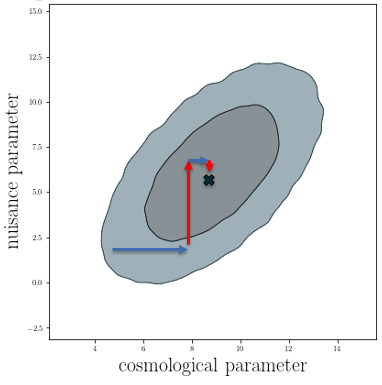
\includegraphics[scale=0.4]{plots/iterative.png}
\caption{Sketch of the iterative fitting method {\color{red} add description here}}
\label{fig:comb}
\end{figure}
\section{Results}
We implement the marginalised likelihood given in Eq. \ref{eq:marginal_likelihood} in the existing KV-450 likelihood, which is publicly available in {\sc MontePython}. We choose priors on cosmological parameters and  nuisance parameters equivalent to the ones in \citetalias{hildebrandt18}. Note that in contrast to the fiducial KV-450 analysis we do not include linear shifts $\delta z_i$ of the mean redshift in each tomographic bin as nuisance parameters since these are replaced by the amplitudes of the gaussian comb. Our choice of priors is reported in Table \ref{tab:priors}.
\begin{table}
\label{tab:priors}
\begin{tabular}{lll}
\hline
Parameter & Symbol & Prior\\
\hline
CDM density & $\Omega_{\rm CDM} h^2$ & $[0.01, 0.99]$\\
Scalar spectrum ampl. & $\ln(10^{10}A_{\rm s})$ & $[1.7, 5.0]$\\
Baryon density & $\Omega_{\rm b} h^2$ & $[0.019, 0.026]$ \\
Scalar spectral index & $n_{\rm s}$ & $[0.7, 1.3]$ \\
Hubble parameter & $h$ & $[0.64, 0.82]$ \\
\hline
IA amplitude & $A_{\rm IA}$ & $[-6, 6]$\\
Baryon feedback amplitude & $B$ & $[2.00, 3.13]$\\
Constant $c$-term offset & $\delta c$ & $0.0000\pm0.0002$ \\
2D $c$-term amplitude & $A_c$ & $1.01\pm0.13$\\
\hline
\end{tabular}
\caption{Model parameters and their priors for the KV450 cosmic shear analysis, adopted from \citetalias{hildebrandt18}. The first five lines are cosmological parameters while the remaining lines represent nuisance parameters. Brackets indicate top-hat priors while values with errors indicate Gaussian priors.}
\end{table}

\subsection{Redshift distribution calibration}
\label{se:redshift_calibration}
As decribed in section \ref{sec:redshift_distribution_model}, we fit a mixture of modified gaussians to the KV450 redshift distributions in five tomographic bins. These distributions were obtained using the fiducial technique, dubbed DIR, which utilizes a direct estimate from deep spectroscopic surveys (see \citetalias{hildebrandt18} for a detailed description). In particular, we simultaneously fit the redshift distributions of all tomographic bins, which are coupled through a correlation matrix that was estimated using a spatial bootstrapping approach. To test the sensitivity of the calibration to the choice of bin width of the input data histograms, we perform the calibration using two different input data histograms: First, we use the histograms with a bin width of $\Delta z = 0.05$ which were used to produce the fiducial result of \citetalias{hildebrandt18}. Secondly, we test a finer binning of the input histograms with a width of $\Delta z = 0.025$. Since we are free to choose the number of gaussian components of the redshift distribution model, we perform several fits with varying number of components. Fit results are reported in Table \ref{tab:redshift_calibration} and a comparison of the two input data histograms is illustrated in Fig. \ref{fig:120vs240}. Comparing the fitted redshift distributions in Fig. \ref{fig:120vs240} we see that the choice of the histogram bin width only has a marginal impact on the fitted curve. However, comparing the goodness of fit which is given in terms of $\chi^2/{\rm d.o.f.}$ in Table \ref{tab:redshift_calibration} we find the model in general provides a bad fit to the data. 
\begin{figure}
\label{fig:120vs240}
\centering
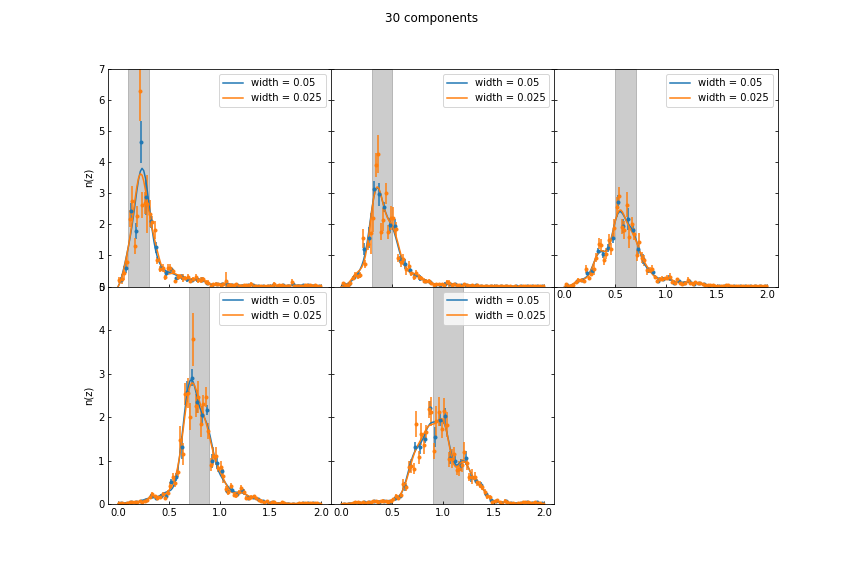
\includegraphics[scale=0.3]{plots/30.png}
\caption{Comparison of redshift distribution calibrated with input data histograms with bin width of $\Delta z = 0.05$ and $\Delta z = 0.025$ {\color{red} change legend!}}
\label{fig:comb}
\end{figure}
\begin{table}
\label{tab:redshift_calibration}
\begin{tabular}{llll}
\hline
dataset & $N_{\rm model}$ & d.o.f. & $\chi^2/{\rm d.o.f.}$\\
\hline
KV-450 DIR&20&20&282\\
$\Delta z = 0.05$&30&10&451\\
$N_{\rm data} = 40$&40&0&n/d\\
\hline
KV-450 DIR&20&60&450\\
$\Delta z = 0.025$&30&50&453\\
$N_{\rm data} = 80$&40&40&567\\
&50&30&683\\
&60&20&996\\
&70&10&1944\\
&80&0&n/d\\
\hline
\end{tabular}
\caption{Fit results of the redshift calibration for two different choices of histogram bin width of the input data. }
\end{table}
The correlation matrix of a fit with 40 fit parameters per redshift bin is presented in Fig. \ref{fig:correlation_matrix}, showing a clear correlation between amplitudes of neighbouring redshift bins.  

As outlined in Section \ref{sec:redshift_distribution_model} we proceed with a further calibration of the redshift distribution using an iterative fitting method of cosmological and nuisance parameters. The fit result for the three most interesting cosmological parameters $A_{IA}$, $\Omega_m$, and $S_8$ are given in Table \ref{tab:iterative_calibration}. 
\begin{table}
\begin{tabular}{lllll}
& $A_{IA}$ & $\Omega_m$ & $S_8$ & $\chi^2$\\
\hline
\hline
fiducial KV450 likelihood & $0.8656$ & $0.2146$ & $0.7708$ & $179.8831$\\
\hline
1. cosmology optimisation & $0.7353$ & $0.2139$ & $0.7768$ & $180.67$\\
2. nuisance optimisation & --- & --- & --- & $179.105$\\
3. cosmology optimisation & $0.7903$ & $0.213$ & $0.7882$ & $178.617$\\
\end{tabular}
\caption{{\color{red} This is a caption}}
\label{tab:iterative_calibration}
\end{table}
\begin{figure}
\centering
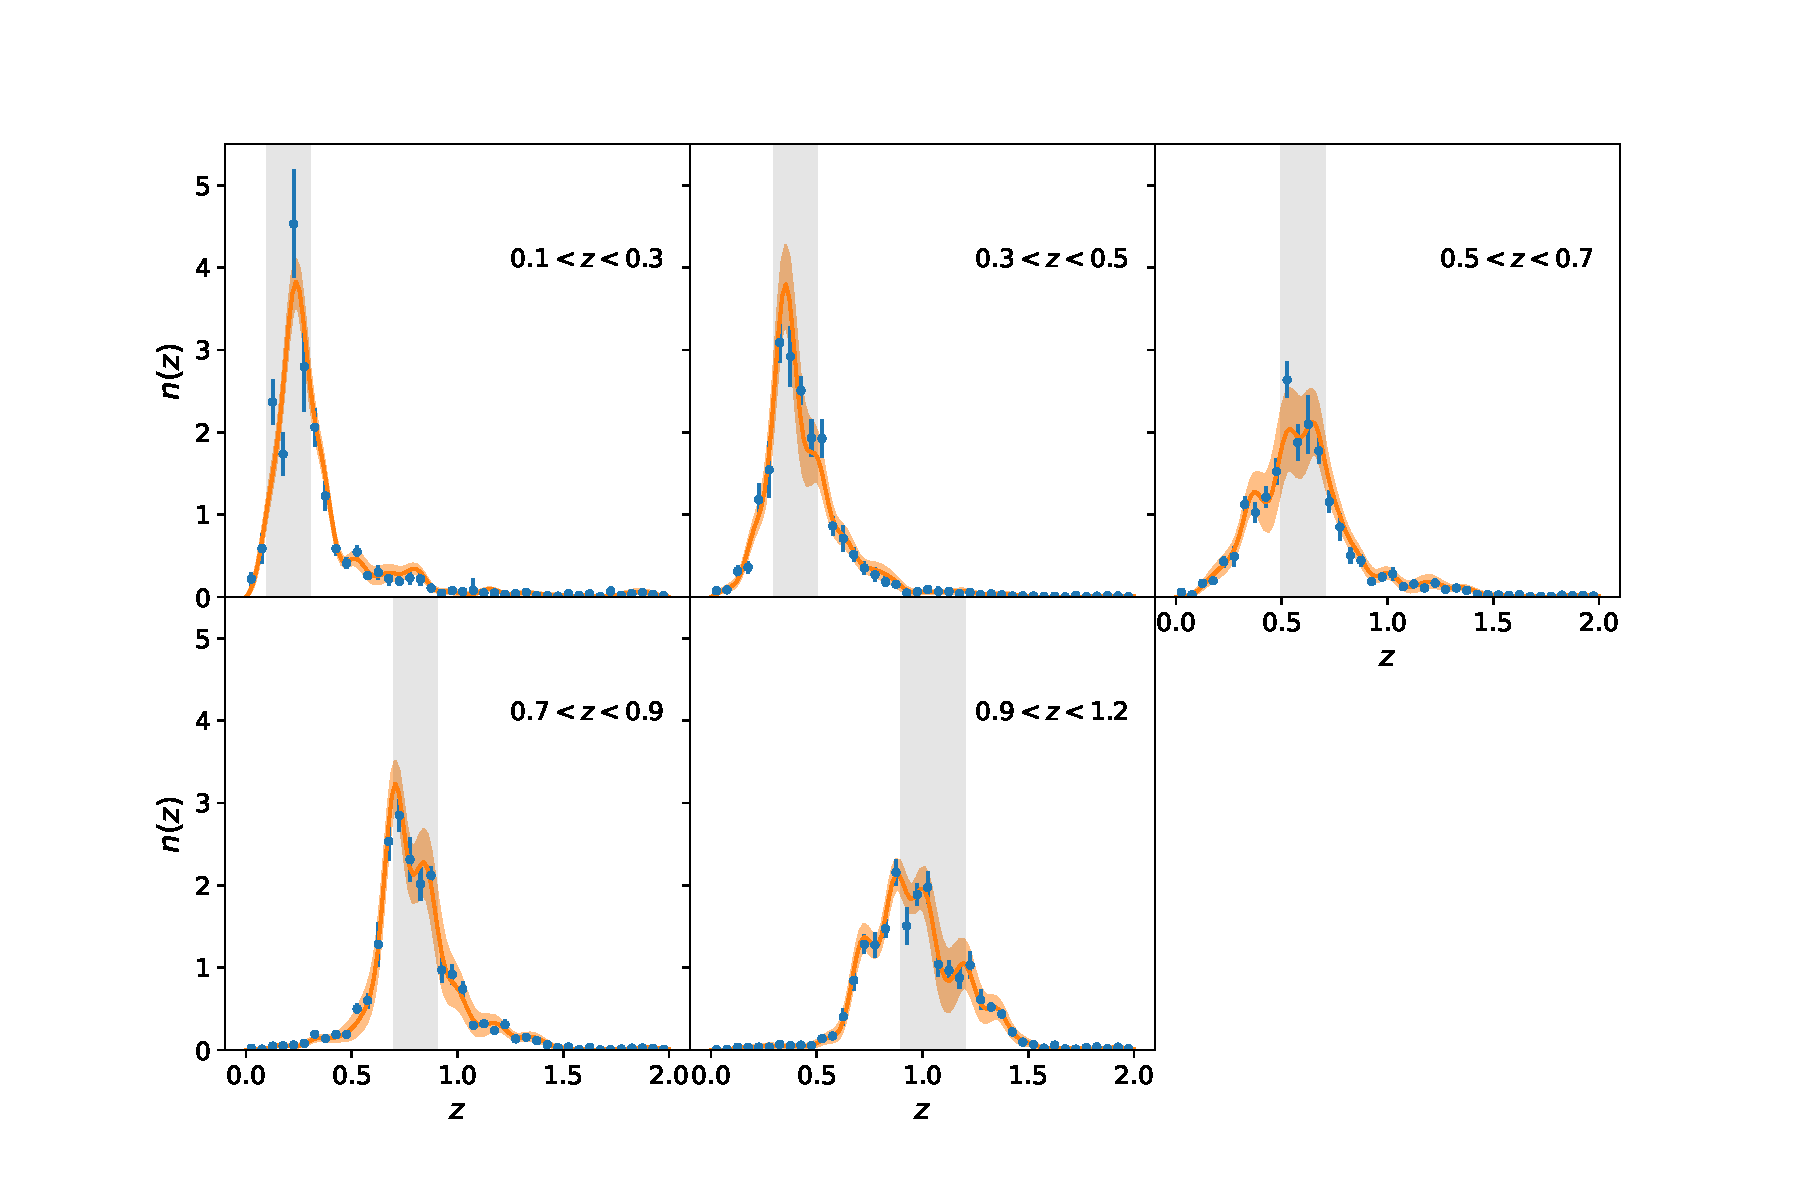
\includegraphics[scale=0.3]{plots/combfit_linear.pdf}
\caption{Fit results of a gaussian mixture with 40 components to the N(z) distribution in 5 tomographic redshift bins. Data is shown in blue and the resulting fit is shown in orange with shaded region indicating the 1$\sigma$ confidence interval.}
\label{fig:comb}
\end{figure}
\begin{figure}
\centering
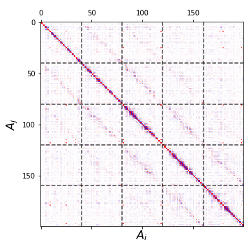
\includegraphics[scale=0.7]{plots/corr.png}
\caption{Correlation matrix of the redshift calibration}
\label{fig:correlation_matrix}
\end{figure}
\subsection{Consistency check}
In order to test if the fitted redshift distribution is capable of reproducing the results of the fiducial KV-450 analysis we sample the likelihood using our redshift distribution model, but without marginalisation over the uncertainty of nuisance parameters. To make a fair comparison of the two likelihoods we fix the nuisance parameters $\delta z_i$ of the KV-450 likelihood. Results of these fits are presented Table \ref{tab:consistency}, showing the constraints on cosmological and nuisance parameters. We find that constraints from both setups are fully consistent and therefore we conclude the the fitted redshift distribution can be used as an alternative to the fiducial redshift histograms.

\begin{figure}
\centering
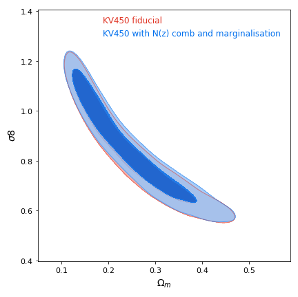
\includegraphics[scale=0.5]{plots/Om_s8.png}
\caption{{\color{red} This is a caption}}
\label{fig:Om_s8_consistency}
\end{figure}

\begin{table}
\begin{tabular}{lll}
\hline
\hline
Parameter & fiducial KV450 & KV450 with comb\\
\hline
$\omega_{cdm }  $ & $0.112^{+0.029}_{-0.060}   $& $0.112^{+0.046}_{-0.060}   $\\

$\ln10^{10}A_{s }$ & $3.30\pm 0.92              $& $3.34\pm 0.92              $\\

$\omega_{b }    $ & $0.0223\pm 0.0021          $& $0.0222^{+0.0018}_{-0.0025}$\\

$n_{s }         $ & $1.03^{+0.15}_{-0.13}      $& $1.01\pm 0.13              $\\

$h              $ & $0.749^{+0.067}_{-0.028}   $& $0.746^{+0.062}_{-0.033}   $\\
\hline
$A_{IA }        $ & $0.89^{+0.64}_{-0.58}      $& $0.70^{+0.64}_{-0.58}              $\\

$c_{min }       $ & $2.50^{+0.22}_{-0.45}      $& $2.49^{+0.23}_{-0.40}     $\\

$dc             $ & $0.00000\pm 0.00019        $& $0.00000\pm 0.00019        $\\

$Ac             $ & $1.03\pm 0.12              $& $1.02\pm 0.12              $\\

$\Omega_{m }    $ & $0.242^{+0.052}_{-0.11}    $& $0.242^{+0.055}_{-0.11}    $\\

$\sigma_8        $ & $0.86^{+0.18}_{-0.20}      $& $0.87\pm 0.17      $\\
\hline
\end{tabular}
\caption{{\color{red} This is a caption}}
\label{tab:consistency}
\end{table}
\subsection{Marginalisation over nuisance parameters} 
In this section we present the main results of our analysis marginalised over the uncertainty on the amplitudes of the fit of the redshift distribution.

%--------------------------------------------------------------------
\section{Conclusions}

  
\begin{acknowledgements}
  
\end{acknowledgements}


\bibliographystyle{aa}
\bibliography{bibliography}


\begin{appendix} 

\section{TBD}


\end{appendix}
%
%
\end{document}
